\documentclass[12pt, a4paper, oneside, openright, medskipamount]{report}

\usepackage{float}
\usepackage{url}
\usepackage{enumitem}
\usepackage{pifont}
\usepackage[utf8]{inputenc}
\usepackage[english]{babel}

\setlength{\parindent}{0em}
\setlength{\parskip}{1em}
\renewcommand{\baselinestretch}{1.1}

\newfloat{fig}{thp}{lof}[chapter]
\floatname{fig}{Figure}

\title{%
Tutorial Builder \\
\large Final Report}

\author{Zoltan Debre}

% Victoria University ECS
\usepackage[image,ecs,mcompsci]{vuwproject}

\supervisor{Dr Stuart Marshall}

% \date{}

\begin{document}

\frontmatter

%%%%%%%%%%%%%%%%%%%%%%%%%%%%%%%%%%%%%%%%%%%%%%%%%%%%%%%

%%%%%%%%%%%%%%%%%%%%%%%%%%%%%%%%%%%%%%%%%%%%%%%%%%%%%%%

\begin{abstract}

Presenting a computer programming problem or solution with a high-quality video is time-consuming and it is not easy to update.

Technical content producers are struggling to find an efficient and interactive way to show their work.

This research introduces a tool that can be used for creating an interactive tutorial.

Furthermore this tool shows programming code snippets in web based code editor so the content creator can build a playable step by step "movie" with it.

\end{abstract}

%%%%%%%%%%%%%%%%%%%%%%%%%%%%%%%%%%%%%%%%%%%%%%%%%%%%%%%

\maketitle

\tableofcontents

%%%%%%%%%%%%%%%%%%%%%%%%%%%%%%%%%%%%%%%%%%%%%%%%%%%%%%%

\mainmatter

%%%%%%%%%%%%%%%%%%%%%%%%%%%%%%%%%%%%%%%%%%%%%%%%%%%%%%%

\chapter{Introduction}

This project is about building an online publishing tool prototype, using code editors and step by step instructions to present programming challenges and solutions for a computer science problem.

The prototype has two parts, an administration area, where the content creator can build a tutorial, and a player tool, where the recorded steps would be presented.

The primary target user is the creator, who composes a new tutorial. The creator can be a teacher, or an open source project owner, who would like to introduce their tool or code.

The secondary user is the consumer, who wants to learn or know more about a problem or a coding solution.

\section{Motivation}

We all have the unstoppable desire to learn. We are keen to know more about the world around us, about our hobby and our profession. In software development, in computer science, the knowledge is essential, it is the key to succeeding. Reading, studying, sharing. An infinite loop of collecting and adapting new practices.

In information technology, especially in programming languages, writing blog posts, creating static, step by step tutorials are a popular way to share or learn something new. Producing and sharing the content is easier nowadays, but still requires more effort from the creator, when they want to deliver an easy to understand high-quality tutorials.

Creating interactive tutorials are appealing, but the production cost is much higher. Recording a video tutorial or especially updating it is time-consuming, and it involves more effort from the creator.

I think an ideal solution would be a healthy mix of static and dynamic contents, where the learners can read instructions but meanwhile they can watch the steps in a code editor, in a more realistic environment.

\section{The problem}

When a developer, teacher or hobbyist would like to present a computer programming problem or solution, most of the times they record a video and publish it on YouTube. Sometimes the easiest way to record a video of a conference/meetup presentation or a live coding session. However recording and editing a high-quality video is time-consuming and less flexible. It is also hard to update.

Other problem with showing tutorials with a simple video, that the audience cannot give it a try, they have to configure their computer and environment to play with the presented solution.

Most of the cases we would like to show instructions and code snippets, mainly text-based contents. It is preferred to show code snippets in a more realistic environment, such as in a code editor. Therefore using the online code editor with a pre-scripted way to play the presentation, where the user can navigate back and forth and can modify or play with the code is more interactive. It involves everyone and helps to understand a problem clearly.

Additionally, it is much easier to maintain, upgrade or fix for the content creator.

Furthermore, the user is able to experience it and can see the result, so the new information can be put into practice immediately.

\section{Personas and their goals}

\subsection{Primary persona}

Content creator, open source project maintainer, teacher.

Their motivation is to present a technical problem and the solution in a clear and an easy-to-understand way. The best option is to show a demo, what happens when we insert the suggested code, how easy it is to use. Most of the times a presentation involves more steps. For example, we would like to show a starting state, maybe a few lines of code which we are able to simplify, so in this case, the first step is to show the problem and after we show step by step how we solve that.

\subsection{Secondary persona}

The consumer, who watch the presentation, who reads the tutorial and who wants to learn more about the actual problem.

They would like to play, stop, and control the presentation. Control the flow, going forward or stepping back.

They would like to try the solution, for example how the final state changes when they modify the code.

\subsection{Target groups}

I develop a prototype web app, where the content producer can create a simple step by step tutorial, and the content consumer can "watch" this tutorial and can interact with it.

There are two different users:
\begin{itemize}[noitemsep]
\item content producer, for example a teacher
\item content consumer, for instance a student
\end{itemize}

\chapter{Related Work}

During the development and research work, I found a few related interesting projects. These are similar or I can use them partly.

\section{CodeMirror Movie}

I found this project when I checked the most popular web-based code editor tool, CodeMirror website. The creator of the CodeMirror wanted to present their tool with a realistic way, so CodeMirror Movie was born. \cite{cm-movie}

This solution highly coupled with CodeMirror, it is similar to an add-on, so it is possible to attach any CodeMirror implementation. (More about CodeMirror in the next section.)

Adding CodeMirror Movie to our project is straightforward because the open source repository provides a CSS and a JS file, so they can be added to any page.

This tool mainly targets web-developers, so with the help of this tool they can add code and scripts to their websites.

Editing "the movie" script is manual. There is a simple syntax which control the presentation steps and this script should be added to the textarea which will be in the code editor.

We clearly see that it is a very effective way to build a presentation, however it requires real development skills.\\

\noindent Pros:
\begin{itemize}[noitemsep]
\item simple, lightweight implementation
\item easy to add your project if you use CodeMirror and you are a developer
\item simple script language to manage the presentation
\item user can use the code editor to try the presented solution
\end{itemize}
Cons:
\begin{itemize}[noitemsep]
\item mainly for developers only
\item highly coupled with CodeMirror
\end{itemize}


\section{Comparison of online code editors}

There are 3 popular web based code editors: CodeMirror, Ace Editor and Monaco.

CodeMirror and Ace Editor are commonly used on websites and different projects. Monaco is a new solution from Microsoft and it is extracted from their popular Microsoft Visual Studio Code developer tool.

There is not significant differences between them. All has the most important code editor features, like supporting more than 100 languages, autocompletion, syntax highlighting, controlling with shortcuts.

I choose CodeMirror, because it has already Ember.js support. Thanks for the ivy-codemirror Ember addon, it can be added to any Ember.js project with the installation of the addon. \\

\noindent CodeMirror
\begin{itemize}[noitemsep]
\item Github link: \url{https://github.com/codemirror/CodeMirror}
\item Website: \url{http://codemirror.net/}
\item Popularity (GitHub Star): 9396
\item Ember.js Addon: \url{https://www.emberobserver.com/addons/ivy-codemirror} \\
\end{itemize}

\noindent Ace Editor
\begin{itemize}[noitemsep]
\item Github link: \url{https://github.com/ajaxorg/ace}
\item Website: \url{https://ace.c9.io}
\item Popularity (GitHub Star): 12950
\item Ember.js Addon: none
\end{itemize}

\noindent Monaco
\begin{itemize}[noitemsep]
\item Github link: \url{https://github.com/Microsoft/monaco-editor}
\item Website: \url{https://microsoft.github.io/monaco-editor/}
\item Popularity (GitHub Star): 2322
\item Ember.js Addon: none
\end{itemize}

\section{Reviewing code sharing websites}

We can use code editor and sharing platforms also when we want to demo a small feature or describe a problem. These websites are combinations of code editors and an iframe where we can see the preview of the code snippets.

One of the common features is splitting the screen and providing different windows for editing html, css and javascript separately.

User can save the edited content also. Most of them can be embed in a blog post or in other website. \\

\noindent Most important findings:
\begin{itemize}[noitemsep]
\item All use Code Mirror as code editor
\item All of them separate the css, html and javascript editing in different screens, but they merge into one file, and preview of this merged html file is possible in an iframe.
\item Saving the different type of code (css, javascript, html) separately.
\end{itemize}

\newpage

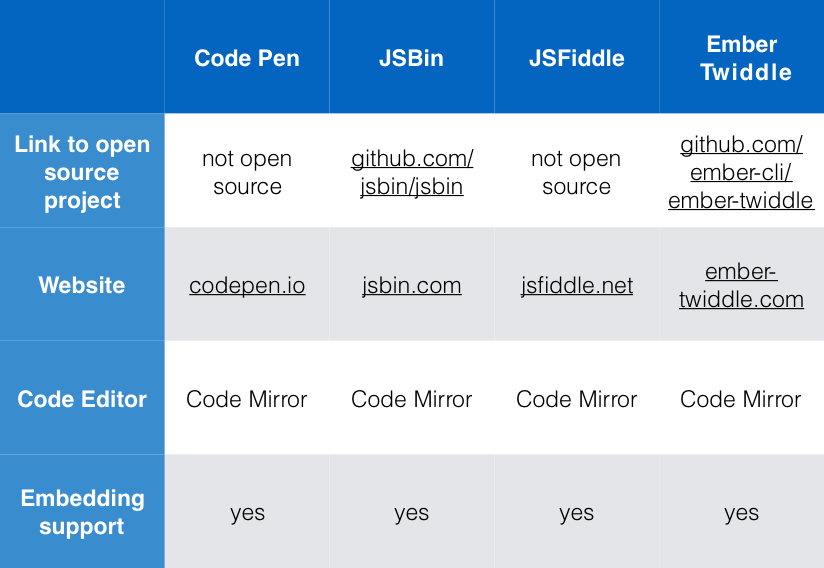
\includegraphics[width=1\textwidth]{assets/code-sharing-website-review}\\*[8pt]

\chapter{Design and Implementation}

\section{The technology of choice}

One of the most popular programming languages in web development is JavaScript. The usage of this frontend focused technology is growing quickly.  It is the 7th on Tiobe Index, which is a good indicator of programming languages popularity. \cite{tiobe}

Learning and teaching JavaScript, HTML and CSS is important. My tool focuses on this three main building blocks of the web.

Building a frontend heavy application, with a dynamic, user-friendly interface is more common nowadays. In the last few years JavaScript based frontend frameworks became mature, production ready tools. Server side technologies, like database management and time and resource heavy processes are separated from the user focused, design driven view layer, which is developed with usage of frontend frameworks.

The most popular tools are Angular.js, React.js and Ember.js. In my project I use Ember.js. It is an "opinionated" framework. Opinionated, convention over configuration driven framework means that developers should follow specific conventions, instead of using a tool freely. A more strict environment helps to adopt best practices and speed up the development process.

Certainly, we still have to store data and information, so we cannot live without backend and server technology. Luckily there are already cloud-based tools for managing databases. I use Firebase, which is a service provided by Google. Firebase is a cloud-based database, document-store solution and easy to integrate with Ember.js.

Additionally, I started to build a traditional backend server application also to support development and experimenting with a real server side and a cloud-based solutions parallel. My preferred technology on backend side is Ruby on Rails, a popular, also opinionated and convention over configuration driven backend framework. However, I added only one model to this backend, because finally I just focused the Firebase implementation.

Following the most modern standard of web applications, I separate the user faced frontend development and the data store, backend development.

The user face frontend application uses Ember.js frontend framework. Ember.js development requires Node.js on the development machine to run the development environment. This development environment helps to run and modify frontend code quickly, and it generates the final, deployable production code also. The production version of the application is only a static website. It means, there is one index.html, two JavaScript files and two CSS files.

\section{Source control management}

I have been using GitHub for managing source code and tracking code changes. Link to repository: \url{https://github.com/zoltan-nz/tutorial-builder}

\section{Frontend features}

The look and feel of the application follows the standard Bootstrap style. Bootstrap is added to the project. I use "sass" version of the Bootstrap, so I can customize it with the modification of the SaSS variables. SaSS is a modern CSS development environment, helps to programmatically modify the CSS.

The home page of the application is only a placeholder. I added a navigation bar with the following links: Home, Builder, Player, Sandboxes, Dashboard.

I implemented a breadcrumb bar also, which helps in navigation.

First, I created a Sandbox area, where I experiment with the CodeMirror code editor and an iFrame, which shows the preview. This Sandbox page contains the editor. When the source code is updated, the preview page automatically shows the generated website. This feature uses Ember.js default two-way bindings capability.

Database management is already implemented. The main adapter is the Firebase adapter, which automatically update data to the Firebase server. Firebase is a real time database. The limited, free to use version is enough for experimenting and for demo.

The secondary adapter is a JSONApi Adapter. JSON Api \cite{jsonapi} is a new standard of data communication format. This is the Ember.js default adapter. This active only when I use the Ruby on Rails based backend system, it is commented out in the production version, because I haven't added all model to the Ruby on Rails app. I keep it there, because the further development of this project will focus on this backend instead of using Firebase.

\section{Static website hosting}

I have been using surge.sh \cite{surge} for static website hosting, so the actual state of the prototype is updated there regularly. Link to the live version: \url{http://tutorial-builder.surge.sh}

\section{Requirements}

A fully functional tutorial service could have the following requirement list. We can separate them in three different groups. One group focuses on requirements for the tutorial creator/admin/teacher, and other group for the consumer/students and a separate group of requirements for user interface considerations.

\noindent Requirements from the teacher perspective:
\begin{itemize}[noitemsep]
\item Teacher can navigate to Admin page.
\item Teacher can create a new tutorial.
\item Teacher can add steps to the tutorial.
\item A step could be four different type:
\begin{itemize}[noitemsep]
\item Instruction type is a text content.
\item Html type, which adds content to the html editor box.
\item Css type, which adds content to the css editor box.
\item JavaScript type, which adds content to the javascript editor box.
\end{itemize}
\item Teacher can modify the content of a step later.
\item Steps always in sync, so the next step always inherit the previous step state.
\end{itemize}

\noindent Requirements from the student perspective:
\begin{itemize}[noitemsep]
\item Student can see a list of tutorials.
\item Student can click on a tutorial and can see the steps.
\item Steps are presented in order.
\item Student can "play" and "watch" the steps.
\item Student can "pause" and step "backward".
\end{itemize}

\noindent User interface requirements:
\begin{itemize}[noitemsep]
\item The tutorial screen has five area:
\item Instruction area.
\item Html code editor textarea.
\item Css code editor textarea.
\item Javascript code editor textarea.
\item Html preview textarea.
\end{itemize}

\noindent The main website has two main section:
\begin{itemize}[noitemsep]
\item Admin page where Teacher can edit tutorials.
\item Tutorials page where Students can select and watch tutorials.
\end{itemize}

\section{Design considerations}

One of the core element of an application is the database and model layer. Determining data entities are an important step of the planning process and help us in the implementation process.

In a fully featured implementation our database structure would be more complex and would cover extended usecases. Firstly, I list a wider model structure, after I will focus on models what I implemented in the prototype.

Most of the web applications has a user and authentication layer, user related information would be stored in "user" model. Keeping it simple the user model would have three fields: username, password, is\_admin. Username and password is the minimum what we need to identify different users. Additionally we have to store wheather the user has administrator privileges or not.

Because of our main problem domain is tutorials, one of the most important model is the entity where we store the different tutorials. So a "tutorial" model would have at least a "name" field. The tutorial model has many "lesson". Each lesson has a "title", a field where we can store the position, the "sort" value, and it has many "steps" also. So the smallest level of this model structure is the "step" model. Step fields: name, type, code, sort.

Simply: Tutorial -\textgreater Lesson -\textgreater Step

The demo app uses this nested model structure in the "Dashboard" section. During the implementation process, my first iteration tried to cover this wider usecase, however, I realized, the challenge is not really on this area.

Finally I created a "builder" model and a "builder-step" model.

Builder model fields: name (string), builderSteps (hasMany)

BuilderStep model fields: builder (belongsTo), sort (number), comment (string), code (string)

With this simplified structure I was able to focus only the implementation of the tutorial and step builder functionality.

This graph summarizes these database tables and models:

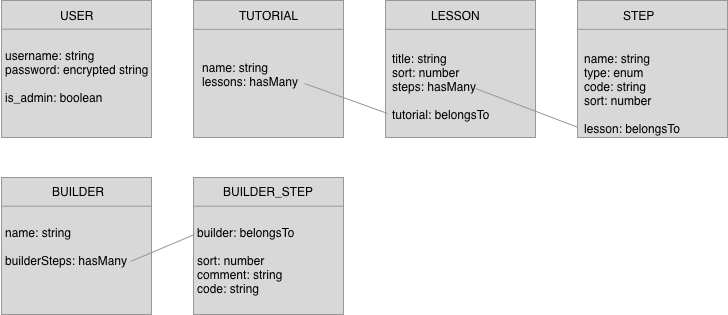
\includegraphics[width=1\textwidth]{assets/database-tables}\\*[8pt]

\section{The story of 12 factor apps}

The Twelve-Factor App is the name of a methodology, which collects together twelve important concepts and rules what we should follow if we build a modern software-as-a-service or web application. We can find this collection on this website: \url{http://12factor.net}

I think, it is important to follow this methodology in our application also, so I bring rules in my prototype implementation from this collection.

Instead of repeating all the 12 rules, I describe how I use a certain rule in my implementation.

1. Codebase. As it already mentioned above, our app uses one codebase, uses git and hosted on Github and the codebase is the same across all deploys.

2. Dependencies. External dependencies of our app managed by a package manager, in our case "npm", the node package manager and "bower", for third party assets, like Ember.js or Bootstrap.

3. Config. The configuration sits separately in "config/environment.js" file, and it could be different on development mode or on production mode.

4. Backing services. The Tutorial Builder backend system is attached via an adapter to the third party database, Firebase, which accessible via a direct URL. This distinct backing service is a resource.

5. Build, release, run. We can build our Ember application with a terminal command "ember build --prod", the production version of the code deployed by an other terminal command "surge" and it is released as production ready.

6. Processes. In our case this rule is relevant also, because our app is a static, single page application, so it is a stateless and "share-nothing" solution.

7. Port binding. This rule would be relevant only if I would use my own server. The backend service and the static single-page application would run from this server using a webserver. In this case the backend server, which could be a Ruby on Rails application, would run on a different port behind the webserver, for example on "http://localhost:3000/" address, however it would be open on the same domain name, but in a subdirectory. For example, if the our Ember.js single-page application would run on "http://tutorial-builder.com/", the Ruby on Rails backend API would be available on "http://tutorial-builder.com/api".

8. Concurrency. Our single page application is stateless, basically a static website. In terms of high traffic, it is easy to clone and launch on more server. Luckily, modern static website hosting services automatically clone it on content delivery network, which means, it can scale out.

9. Disposability. We don't have to turn off our web application, we can just deploy and overwrite the previous version in a second, so the next user will download the updated version.

10. Dev/prod parity. As a twelve-factor developer, it is important for me, that I should be able to deploy continously. It means, I can manage the code, update or fix it, test on the developer machine, test with the production database, build the production version and deploy immediately. With my development environment and with tools of my choice, this principal is adopted also.

11. Logs. This feature can be adopted in our environment, but it is not active in our experimental project.

12. Admin processes. Our database administration focuses only for maintaining, deleting the Firebase database, it can be done on Firebase website as a single process.

\section{Data down actions up}

In software architecture, and computer science it is always a challenge, how could you write clean code \cite{clean-code}, which is always readable and easy to maintain. I built my project mainly in JavaScript, and it is known that JavaScript is not so strickt language, no strick types as in Java, it doesn't force structured object oriented patterns. However, JavaScript changed a lot in the last few years, thanks for the new version. The new JavaScript standard called ES2015 or ES6 \cite{es6}.

JavaScript with ES6 syntax and with a heavily object orinted JavaScript framework, like Ember.js, can force you to write an easy to understand, easy to maintain system. Ember.js is a Model-View-Controller type framework and it helps to separate concerns and make your code more SOLID \cite{solid}.

With modern JavaScript frameworks we mainly build frontend, user faced applications, so the view layer of our product is a webpage or a web component. These pages or components are a mix of static and dynamic content. Static content is built in the presentation template, however the dynamic content usually provided by a backend service from a database.

Modern JavaScript frameworks are adopted a new pattern, which determines the data flow inside the application. It is driven by the user interaction. When a user opens a web application and navigates inside this webapp, usually the browser changes the actual web address in the location bar. We call it "routing". So when the route changes, mainly we navigate to a new page. We usually call it, the "state" of the application is changed. It triggers a series of steps. One of the most important step, that the app tries to access to dynamic data which will be rendered on the page. This data can come from an allready cached local data store or can send an AJAX request to the backend system and download it. After this data rendered on the page.

On a website the previously prepoluated data can change, for example in a web form we change a text in the text field, or change a code in a web based code editor, or the user click on a button, which turns on or off an information. Each case we actually change the data.

Originally web frameworks are introduced a uniqe concept, which is called two-way bindings. When data change somewhere in the application, it broadcasted everywhere, so quite quickly we were able to build a dynamic web application. In our project, when a user edits code in the code editor, the preview window automatically updates, because the code is change in that IFRAME also.

Two-way binding has own benefits and use cases. It is very usefull when we use data in the same context (same page, same object oriented class in our code). However, two-way bindings can cause data leak, so when we change something on the page, an unexpected behaviour could happen. It can be easily managed in a small application, but when our application grows, very difficult to maintain.

For this reason, there is this new pattern, what we call "data down actions up". It is prefered to turning off the two-way binding in the application and keep the automatic update in a small scope only. When we want to populate the new data, it could be calling with a direct function in our app. It is called actions. So instead of letting the invisible "magic" update states in our application, we clearly call and send actions to the other part of the app.

The benefit of this, if someone else try to understand our code, there is not any invisible part.

\section{Low level design decisions}

- Managing css with sass and adding bootstrap.

- Code mirror plugin

- Bread crumbs





\subsection{Communication between two components}

- Adding ember-wormhole

\section{Challenges}

Database management:
- using mock (mirage)
- using ruby on rails backend
- keeping only Firebase


\section{Reflection}

- Great part
- Need improvement
- Would do differently?

\chapter{Evaluation}

\section{Process}

The product evaluation has two parts. The first part is expert evaluation, which means, I collected feedbacks from my direct colleagues (from my workplace and from research group). The second part is a survey, which helped to collect opinion about programming tutorial usage.

\subsection{Expert evaluation}

Expert evaluation helps to discover quickly the "low-hanging fruits", obvious usability problems, without investing extra resource for a wide user testing.

My reserach product is a prototype, which cannot be perfect for the first iteration, but already can help us to direct our future study.

Feedbacks from experts:

* Deleting a tutorial step is confusing, because

\subsection{Tutorial Builder Survey}

Watching, reading or following tutorials are important part of our learning process, but everybody could have different motivation. I launched a survey for collecting information about user's motivation and their goal.

Victoria University ethics committee approved my request, so I run a little campaign on my twitter, on my blog and shared the link in different developer chat groups.

I built the survey on Google Survey platform, and it was presented as the following screenshot shows.

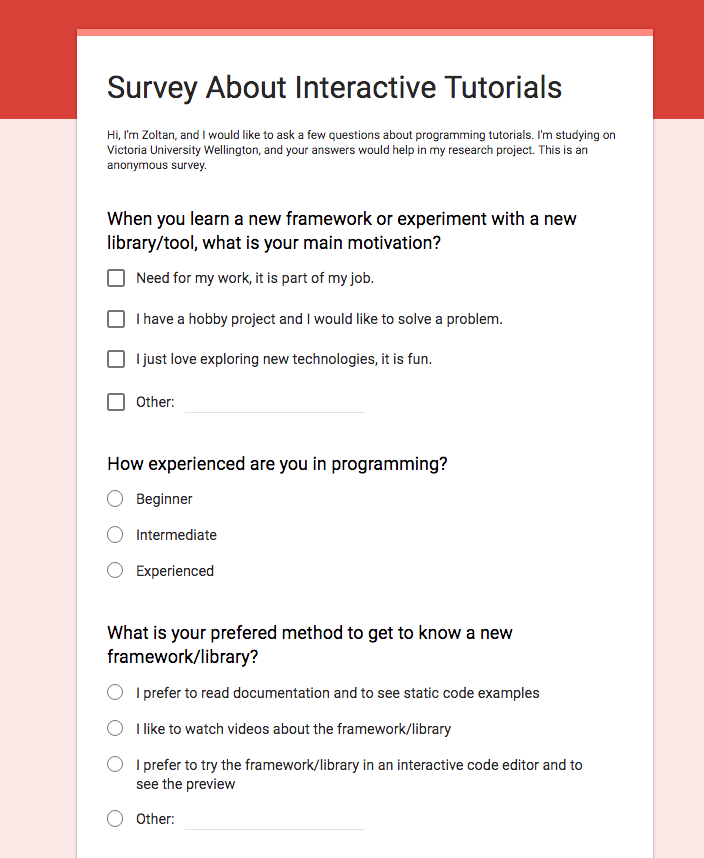
\includegraphics[width=1\textwidth]{assets/survey-screenshot.png}\\*[8pt]

\textbf{The questions and options:}

\noindent When you learn a new framework or experiment with a new library/tool, what is your main motivation?
\begin{itemize}[noitemsep]
\item Need for my work, it is part of my job
\item I have a hobby project and I would like to solve a problem.
\item I just love exploring new technologies, it is fun.
\item Other...
\end{itemize}

\noindent How experienced are you in programming?
\begin{itemize}[noitemsep]
\item Beginner
\item Intermediate
\item Experienced
\end{itemize}

\noindent What is your prefered method to get to know a new framework/library?
\begin{itemize}[noitemsep]
\item I prefer to read documentation and to see static code examples
\item I like to watch videos about the framework/library
\item I prefer to try the framework/library in an interactive code editor and to see the preview
\end{itemize}

\noindent When you try a library or a framework in a web based code editor, which features are important to you? (Scale from 1-not important to 6-very important)
\begin{itemize}[noitemsep]
\item There is a step by step introduction of the usage of the library
\item I can pause, reverse the introduction
\item I can modify the code in the web based code editor
\item I can share/export/copy the code from the web based code editor
\end{itemize}

What other features would you like to see in a web based interactive tutorial.
(open question)

I got 68 answers.

The results from the survey.

\includegraphics[width=1\textwidth]{assets/survey-Q1.png}\\*[8pt]

... More pictures

It was great to see how many suggestions arrived for the open question.

Most importants:

...
...




\section{Analysis}

\chapter{Conclusion}



%%%%%%%%%%%%%%%%%%%%%%%%%%%%%%%%%%%%%%%%%%%%%%%%%%%%%%%

\backmatter

%%%%%%%%%%%%%%%%%%%%%%%%%%%%%%%%%%%%%%%%%%%%%%%%%%%%%%%

\bibliographystyle{acm}

\begin{thebibliography}{9}

\bibitem{tiobe}
Tiobe.com - \url{http://www.tiobe.com/tiobe_index}

\bibitem{cm-movie}
CodeMirror Movie - \url{https://github.com/sergeche/codemirror-movie}

\bibitem{jsonapi}
JSON Api - \url{http://jsonapi.org}

\bibitem{surge}
Surge.sh Static Website Hosting Service - \url{http://surge.sh}

\bibitem{clean-code}
Book: Robert C. Martin - Clean Code - ISBN-13: 978-0132350884

\bibitem{es6}
ES6 Standard - \url{http://www.ecma-international.org/ecma-262/6.0/}

\bibitem{solid}
SOLID pattern - \url{https://en.wikipedia.org/wiki/SOLID_(object-oriented_design)}

\end{thebibliography}

%%%%%%%%%%%%%%%%%%%%%%%%%%%%%%%%%%%%%%%%%%%%%%%%%%%%%%%

\end{document}

